\documentclass[../../main.tex]{subfiles}

\begin{document}
	Im letzten Kapitel hast du einige wichtige bekannte Zahlenmengen kennengelernt, die natürlichen, ganzen, rationalen und die reellen Zahlen. Diese Mengen können wir verwenden, um andere Mengen, etwa die Menge der geraden Zahlen, elegant zu notieren. Mit einer weiteren wichtigen Art von Mengen wollen wir uns im Folgenden beschäftigen, den sogenannten \textbf{Intervallen}.
	
	Ein Intervall ist eine Teilmenge der reellen Zahlen. Wie im letzten Kapitel können wir uns die reellen Zahlen \Real als Zahlenstrahl vorstellen. Ein Intervall ist dann ein zusammenhängender Abschnitt auf diesem Zahlenstrahl.
	
	\begin{figure}[h]
		\centering
		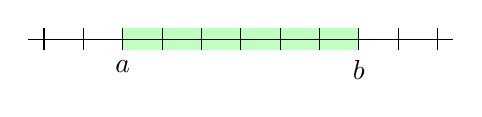
\begin{tikzpicture}
			\fill [green!25] (1,-4pt) rectangle (4,4pt);
			\draw (-0.2,0)--(5.2,0);
			\foreach \x in {0,0.5,1,...,5} {
				\draw (\x,4pt)--(\x,-4pt);
			}
			\node[below] at (1,-4pt) {$a$};
			\node[below] at (4,-4pt) {$b$};
		\end{tikzpicture}
		\caption{Der grün markierte Abschnitt gibt ein Intervall an, das die Zahlen $a$, $b$ und alle dazwischen liegenden enthält. Formal besteht aus allen Zahlen $x \in \Real$ mit $a \leq x \leq b$.}
	\end{figure}

	Zusammenhängend heißt, dass dieser Abschnitt keine Lücken enthalten darf. Die markierten Bereiche im unteren Bild bilden zusammen zum Beispiel kein Intervall.
	
	\begin{figure}[h]
		\centering
		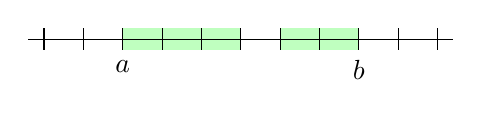
\begin{tikzpicture}
			\fill [green!25] (1,-4pt) rectangle (2.5,4pt);
			\fill [green!25] (3,-4pt) rectangle (4,4pt);
			\draw (-0.2,0)--(5.2,0);
			\foreach \x in {0,0.5,1,...,5} {
				\draw (\x,4pt)--(\x,-4pt);
			}
			\node[below] at (1,-4pt) {$a$};
			\node[below] at (4,-4pt) {$b$};
		\end{tikzpicture}
		\caption{Im grünen Abschnitt befindet sich eine Lücke. Daher wird hier kein Intervall von $a$ nach $b$ dargestellt.}
	\end{figure}
	
	Ein Intervall hängt wesentlich von seinen Endpunkten ab. Im ersten Bild waren dies die Zahlen $a$ und $b$, die jeweils selbst im Intervall enthalten waren. Ein solches Intervall nennt man \textbf{abgeschlossenes Intervall} und wir schreiben dafür $[a,b]$. 
	
	Möchten wir hingegen die Endpunkte aus dem Intervall ausschließen, so schreiben wir stattdessen $(a,b)$. Dies nennt man ein \textbf{offenes Intervall}. Es besteht also aus allen Zahlen, die echt größer als $a$ und echt kleiner als $b$ sind. Das sind alle Zahlen, die auf dem Zahlenstrahl zwischen den Endpunkten $a$ und $b$ liegen, außer den Endpunkten selbst.
	
	\begin{figure}[h]
		\centering
		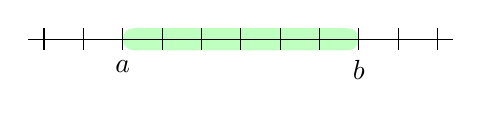
\begin{tikzpicture}
			\fill [green!25, rounded corners] (1,-4pt) rectangle (4,4pt);
			\draw (-0.2,0)--(5.2,0);
			\foreach \x in {0,0.5,1,...,5} {
				\draw (\x,4pt)--(\x,-4pt);
			}
			\node[below] at (1,-4pt) {$a$};
			\node[below] at (4,-4pt) {$b$};
		\end{tikzpicture}
		\caption{Der grüne Abschnitt gibt das Intervall zwischen den Zahlen $a$ und $b$ an. Die abgerundeten Ecken verdeutlichen, dass die Endpunkte nicht im Intervall enthalten sind. Das Intervall besteht somit aus allen $x \in \Real$ mit $a < x < b$.}
	\end{figure}

	Diese beiden Formen können wir auch mischen. Es ist also möglich, ein Intervall anzugeben, das nur einen der beiden Endpunkte enthält. Diese Intervalle nennt man \textbf{halboffene Intervalle}. Wir unterscheiden hierbei zwischen dem \textbf{rechtsoffenem Intervall} $[a,b)$, das den Endpunkt $a$, aber nicht $b$ enthält, und dem \textbf{linksoffenem Intervall} $(a,b]$, bei dem es sich umgekehrt verhält.
	
	\begin{figure}[h]
		\centering
		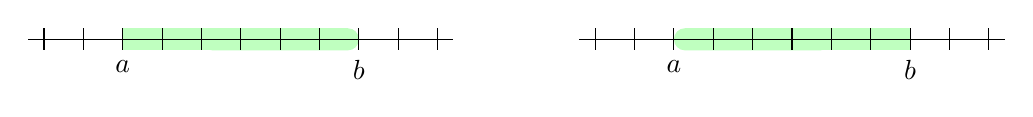
\begin{tikzpicture}
			\begin{scope}[name = rechtsoffen]
				\fill [green!25] (1,-4pt) rectangle (3,4pt);
				\fill [green!25, rounded corners] (2,-4pt) rectangle (4,4pt);
				\draw (-0.2,0)--(5.2,0);
				\foreach \x in {0,0.5,1,...,5} {
					\draw (\x,4pt)--(\x,-4pt);
				}
				\node[below] at (1,-4pt) {$a$};
				\node[below] at (4,-4pt) {$b$};
			\end{scope}
		
			\begin{scope}[right of = rechtsoffen, xshift = 6cm]
				\fill [green!25, rounded corners] (1,-4pt) rectangle (3,4pt);
				\fill [green!25] (2,-4pt) rectangle (4,4pt);
				\draw (-0.2,0)--(5.2,0);
				\foreach \x in {0,0.5,1,...,5} {
					\draw (\x,4pt)--(\x,-4pt);
				}
				\node[below] at (1,-4pt) {$a$};
				\node[below] at (4,-4pt) {$b$};
			\end{scope}
		\end{tikzpicture}
		\caption{Ein rechtsoffenes Intervall (links) und ein linksoffenes Intervall (rechts). Das rechtsoffene Intervall enthält alle $x \in \Real$ mit $a \leq x < b$ und das linksoffene alle $x \in \Real$ mit $a < x \leq b$.}
	\end{figure}
	
	\todo{Beispiel ist noch nicht so richtig geil}
	\begin{example}{}
		\begin{itemize}
			\item $[1,\infty)$ ist die Menge der positiven reellen Zahlen. 
			\item $(-\infty,\infty) = \Real$ ist der gesamte Zahlenstrahl, also die Menge der reellen Zahlen.
			\item $[2,7) \cap \Integer = \{2,3,4,5,6\}$ ist die Menge der ganzen Zahlen von $2$ bis $6$. Diese Menge selber ist kein Intervall, da es nicht die reellen Zahlen zwischen ihren Elementen enthält. Auf dem Zahlenstrahl wären dies Lücken. 
			\item $[3,2] = \left\{ x \in \Real \mid 3 \leq x \leq 2\right\} = \emptyset$ ist die leere Menge, da es keine Zahlen gibt, die größer gleich $3$, aber kleiner oder gleich $2$ sind.
			\item $[5,5] = \left\{ x \in \Real \mid 5 \leq x \leq 5\right\} = 5$, da die einzige Zahl, die größer oder gleich und kleiner oder gleich $5$ die $5$ selbst ist.
		\end{itemize}
	\end{example}

	\begin{definition}{Intervalle}
		Ein \textbf{Intervall} ist eine Teilmenge der reellen Zahlen, die aus allen Zahlen zwischen zwei vorgegebenen reellen Endpunkten $a$ und $b$ besteht. Wir unterscheiden die folgenden Fälle.
		\begin{itemize}
			\item Das \textbf{abgeschlossene Intervall} $[a,b] = \left\{ x \in \Real \mid a \leq x \leq b\right\}$ enthält zusätzlich beide Endpunkte.
			\item Das \textbf{offene Intervall} $(a,b) = \left\{ x \in \Real \mid a < x < b\right\}$ enthält die Endpunkte nicht.
			\item Das \textbf{rechtsoffene Intervall} $[a,b) = \left\{ x \in \Real \mid a \leq x < b\right\}$ enthält zusätzlich  den linken Endpunkt.
			\item Das \textbf{linksoffene Intervall} $(a,b] = \left\{ x \in \Real \mid a < x \leq b\right\}$ enthält zusätzlich den rechten Endpunkt.
		\end{itemize}
	\end{definition}

	
	Die Notwendigkeit von (halb-)offenen Intervallen zu sprechen liegt in den reellen Zahlen selbst begründet. Da wir auf dem Zahlenstrahl mit jedem Punkt, den wir uns aussuchen, auch eine reelle Zahl treffen, können wir beliebig nahe an eine vorgegebene Zahl heranrücken. Das bedeutet, dass wir ein (halb-)offenes Intervall niemals als abgeschlossenes Intervall notieren können, da wir keine passenden Endpunkte angeben können. Diesen Zusammenhang verdeutlicht das folgende Beispiel.
	
	\begin{example}{}
		\parpic[r]{
			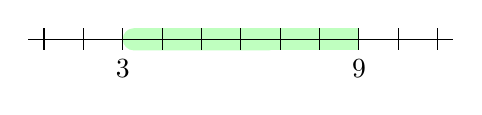
\begin{tikzpicture}
				\fill [green!25, rounded corners] (1,-4pt) rectangle (3,4pt);
				\fill [green!25] (2,-4pt) rectangle (4,4pt);
				\draw (-0.2,0)--(5.2,0);
				\foreach \x in {0,0.5,1,...,5} {
					\draw (\x,4pt)--(\x,-4pt);
				}
				\node[below] at (1,-4pt) {$3$};
				\node[below] at (4,-4pt) {$9$};
			\end{tikzpicture}
		}
		Wir betrachten das linksoffene Intervall $(3,9]$. Dieses besteht aus allen reellen Zahlen, die größer als $3$, aber nur höchstens so groß wie $9$ sind. So enthält es etwa die Zahlen $4$, $7$ und $5.3$. Aber auch die Zahlen $3.1$, $3.01$, $3.001$ und so weiter sind in $(3,9]$ enthalten. Für jede Zahl im Intervall, die nur ein bisschen rechts von der $3$ liegt, finden wir also eine andere Zahl, die noch dazwischen passt. Wir können dieses Intervall also nicht als abgeschlossenes aufschreiben, weil es immer Zahlen gibt, die zwischen der $3$ und dem linken Endpunkt einer möglichen abgeschlossenen Darstellung liegen.
	\end{example}
	
	\begin{example}{Körpergrößen}
		Beispiel, bei dem wir Mengen bilden mit Personen, deren Körpergröße zwischen 163cm und 178cm liegt. Dazu auch alle Fälle für abgeschlossen/halboffen aufschreiben. Wirklich machen? Wenn ja, hier hin?
	\end{example}

	\begin{nutshell}{Intervalle}
		Hier alles zusammenfassen.
	\end{nutshell}
\end{document}
